\subsection{Normal Log-PDF}

\begin{figure*}[t]
    \centering
    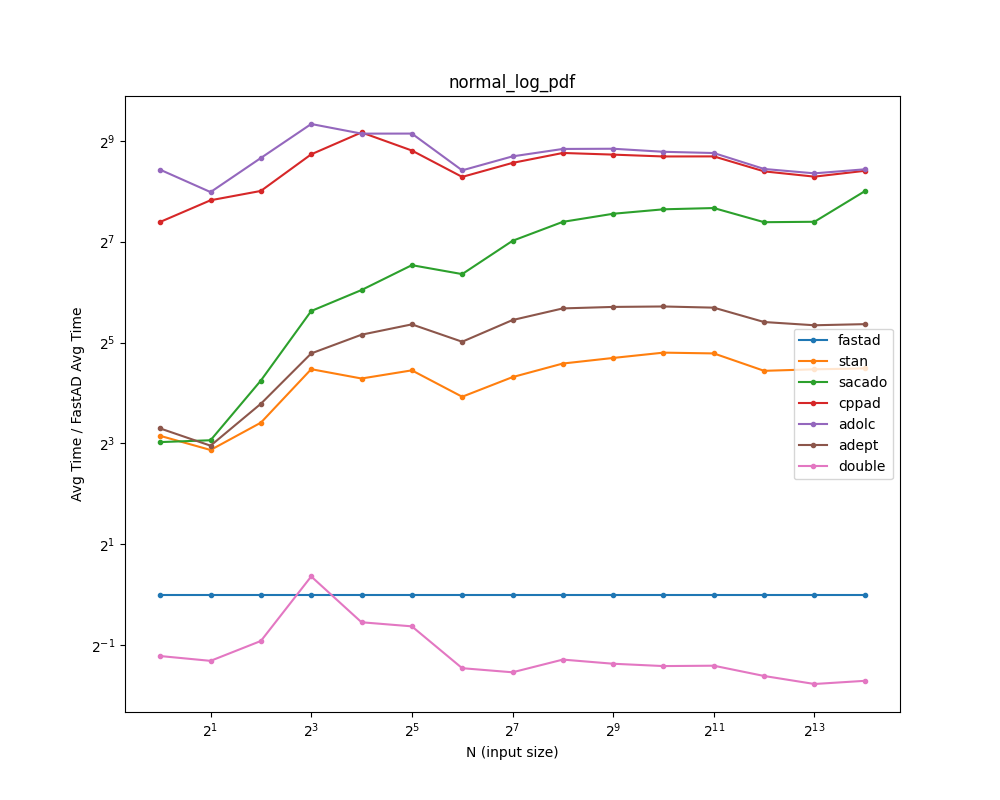
\includegraphics[width=\textwidth]{figs/normal_log_pdf_fig.png}
    \caption{%
        Normal log-pdf benchmark of other libraries against FastAD 
        plotted relative to FastAD average time.
    }\label{fig:normal_log_pdf}
\end{figure*}

The normal log-pdf function is defined up to a constant:
\[
    f(x) = -\frac{1}{2} \sum\limits_{i=1}^N \paren{\frac{x_i - \mu}{\sigma}}^2 
           -N\log(\sigma)
\]
For this benchmark, $\mu = -0.56,\,\sigma = 1.37$ and are kept as constants;
the values themselves are not so important so long as $\sigma > 0$.
Only Stan and FastAD provide built-in functions to compute this function.
All other libraries are written with the \verb|Eigen| API to compute the sum in $f$ except Adept.
Adept provides \verb|norm2| function and we attempted to try the following:
\begin{lstlisting}[style=customcpp]
    adept::aReal operator()(const adept::aVector& x) const
    {
        return -adept::norm2(x - mu_) / (2 * sigma_ * sigma_) 
                - (x.size() * std::log(sigma_));
    }
\end{lstlisting}
however, this does not produce the correct adjoints.
Hence, since Adept does not interface well with \verb|Eigen|~\cite{hogan:2014}, 
our only choice was to write a naive for-loop method.
Fig.\ref{fig:normal_log_pdf} shows the benchmark results.

FastAD is the fastest library for all values of $N$.
It is not surprising that Stan is the next fastest, 
since the Stan Math Library was written precisely for differentiating probability densities.
It is, however, surprising that Adept is the third fastest,
given that we wrote our own for-loop to implement its overload.
The trend stabilizes towards at around $N=2^{7}=128$,
and towards the end
Stan is about $ 22$ times slower,
Adept about $ 41$ times,
and Sacado about $ 198$ times.
